\documentclass[final]{beamer}

% ============================================================
% PLANTILLA DE POSTER CIENTIFICO - beamerposter
% Proyecto: Segmentacion de caries en radiografias panoramicas con CNN
% Formato: A0 vertical, UNA sola columna (sin divisiones).
% ============================================================

\usepackage[size=a0,orientation=portrait,scale=1.15]{beamerposter}
\usetheme{Madrid}

\usepackage[utf8]{inputenc}
\usepackage[spanish]{babel}
\usepackage{graphicx}
\usepackage{booktabs}
\usepackage{amsmath}
\usepackage{tikz}

% ---------- Paleta de colores (tonos azul/salud, ajustable) ----------
\definecolor{colorprincipal}{RGB}{0,90,140}
\definecolor{colorsecundario}{RGB}{0,150,170}
\definecolor{colorfondo}{RGB}{245,248,250}

\setbeamercolor{block title}{fg=white,bg=colorprincipal}
\setbeamercolor{block body}{fg=black,bg=colorfondo}

\setbeamertemplate{block begin}{
  \begin{beamercolorbox}[rounded=true,shadow=false]{block title}
    \vskip0.3ex
    \centerline{\usebeamerfont{block title}\insertblocktitle}
    \vskip0.3ex
  \end{beamercolorbox}
  \vskip-0.05ex
  \begin{beamercolorbox}[rounded=true]{block body}
}
\setbeamertemplate{block end}{
  \end{beamercolorbox}
  \vskip0.5ex
}

% Se desactiva el encabezado por defecto de beamerposter: se construye
% un encabezado propio (logos + titulo + autor + matricula) al inicio del frame.
\setbeamertemplate{headline}{}

\begin{document}
\begin{frame}[t]

% ============================================================
% ENCABEZADO PERSONALIZADO: logo izquierdo, titulo/autor/matricula, logo derecho
% ============================================================
\begin{center}
\begin{tikzpicture}
\node[anchor=west] at (0,0) {%
  % ---- logo de la universidad ----
  \fbox{\parbox[c][6cm][c]{6cm}{\centering 
\includegraphics[width=6cm]{logo_universidad.png}}}
};
\node[anchor=east] at (\linewidth,0) {%
  % ---- logo de la facultad ----
  \fbox{\parbox[c][6cm][c]{6cm}{\centering 
\includegraphics[width=6cm]{logo_facultad.png}}}
};
\node[anchor=center,text width=0.65\linewidth,align=center] at (0.5\linewidth,0) {%
  {\Huge\bfseries\color{colorprincipal} Segmentación de caries en radiografías panorámicas dentales mediante redes neuronales convolucionales}\\[0.6cm]
  {\LARGE Sonia Torres Ibarra}\\[0.2cm]
  {\Large Matrícula: 1563824}\\[0.2cm]
  {\large Maestría en Ciencia de Datos --- Procesamiento y Clasificación de Datos}
};
\end{tikzpicture}
\end{center}

\vspace{1cm}

% ============================================================
% CONTENIDO: una sola columna, todos los bloques apilados
% ============================================================
\begin{columns}[t]
\begin{column}{.92\linewidth}

\begin{block}{Introducción}
Las caries dentales son una de las patologías más frecuentes en odontología.
Su identificación manual en radiografías panorámicas es lenta y depende de
la experiencia del especialista. Este trabajo propone un modelo de
\textbf{segmentación semántica basado en CNN} para delimitar automáticamente
las regiones con caries, aportando información espacial precisa en lugar de
una simple etiqueta de clasificación.
\end{block}

\begin{block}{Objetivo}
Diseñar, entrenar y evaluar una red neuronal convolucional capaz de
segmentar regiones con caries en radiografías panorámicas dentales,
aplicando \textit{transfer learning} y \textit{fine-tuning}.
\end{block}

\begin{block}{Conjunto de datos}
Dataset público \textbf{MLUA} (Wang et al., 2023), con radiografías
panorámicas dentales y sus máscaras de segmentación de caries
(\textit{ground truth}).

\begin{itemize}
  \item Imágenes utilizadas: 100 imágenes
  \item División entrenamiento / validación: 80\% / 20\%
  \item Tamaño de entrada: 224 $\times$ 224 píxeles
\end{itemize}

\vspace{0.5cm}
\begin{center}
% ---- Imagenes de placas  ----
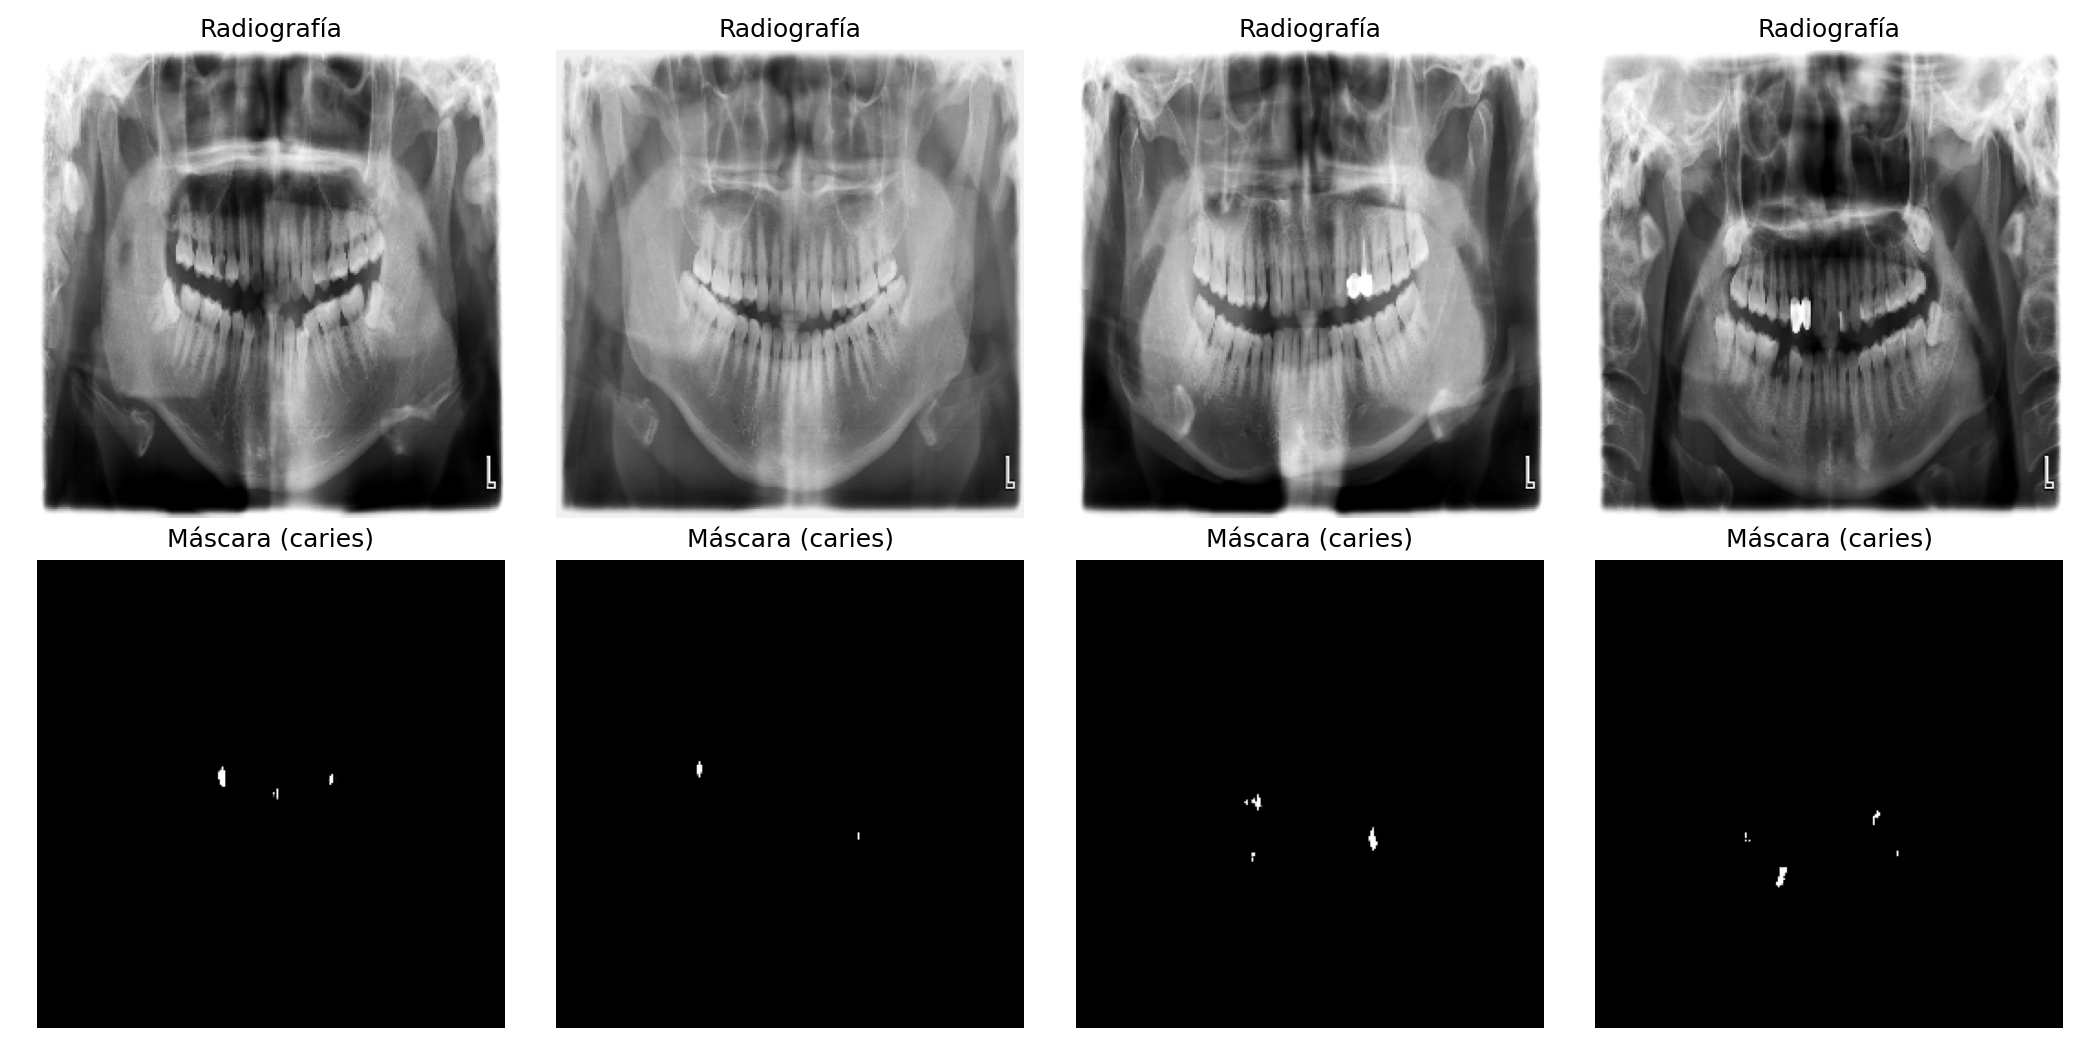
\includegraphics[height=10cm]{radiografia_mascara.png}
\end{center}
\end{block}

\begin{block}{Metodología}

\textbf{Arquitectura: U-Net con encoder VGG16 (transfer learning)}
\begin{itemize}
  \item \textit{Encoder}: VGG16 preentrenado en ImageNet, congelado inicialmente.
  \item \textit{Decoder}: bloques \texttt{Conv2DTranspose} + \textit{skip connections} + convoluciones, entrenado desde cero.
  \item Capa de salida: convolución $1\times1$ con activación sigmoide.
\end{itemize}

\vspace{0.3cm}
\begin{center}
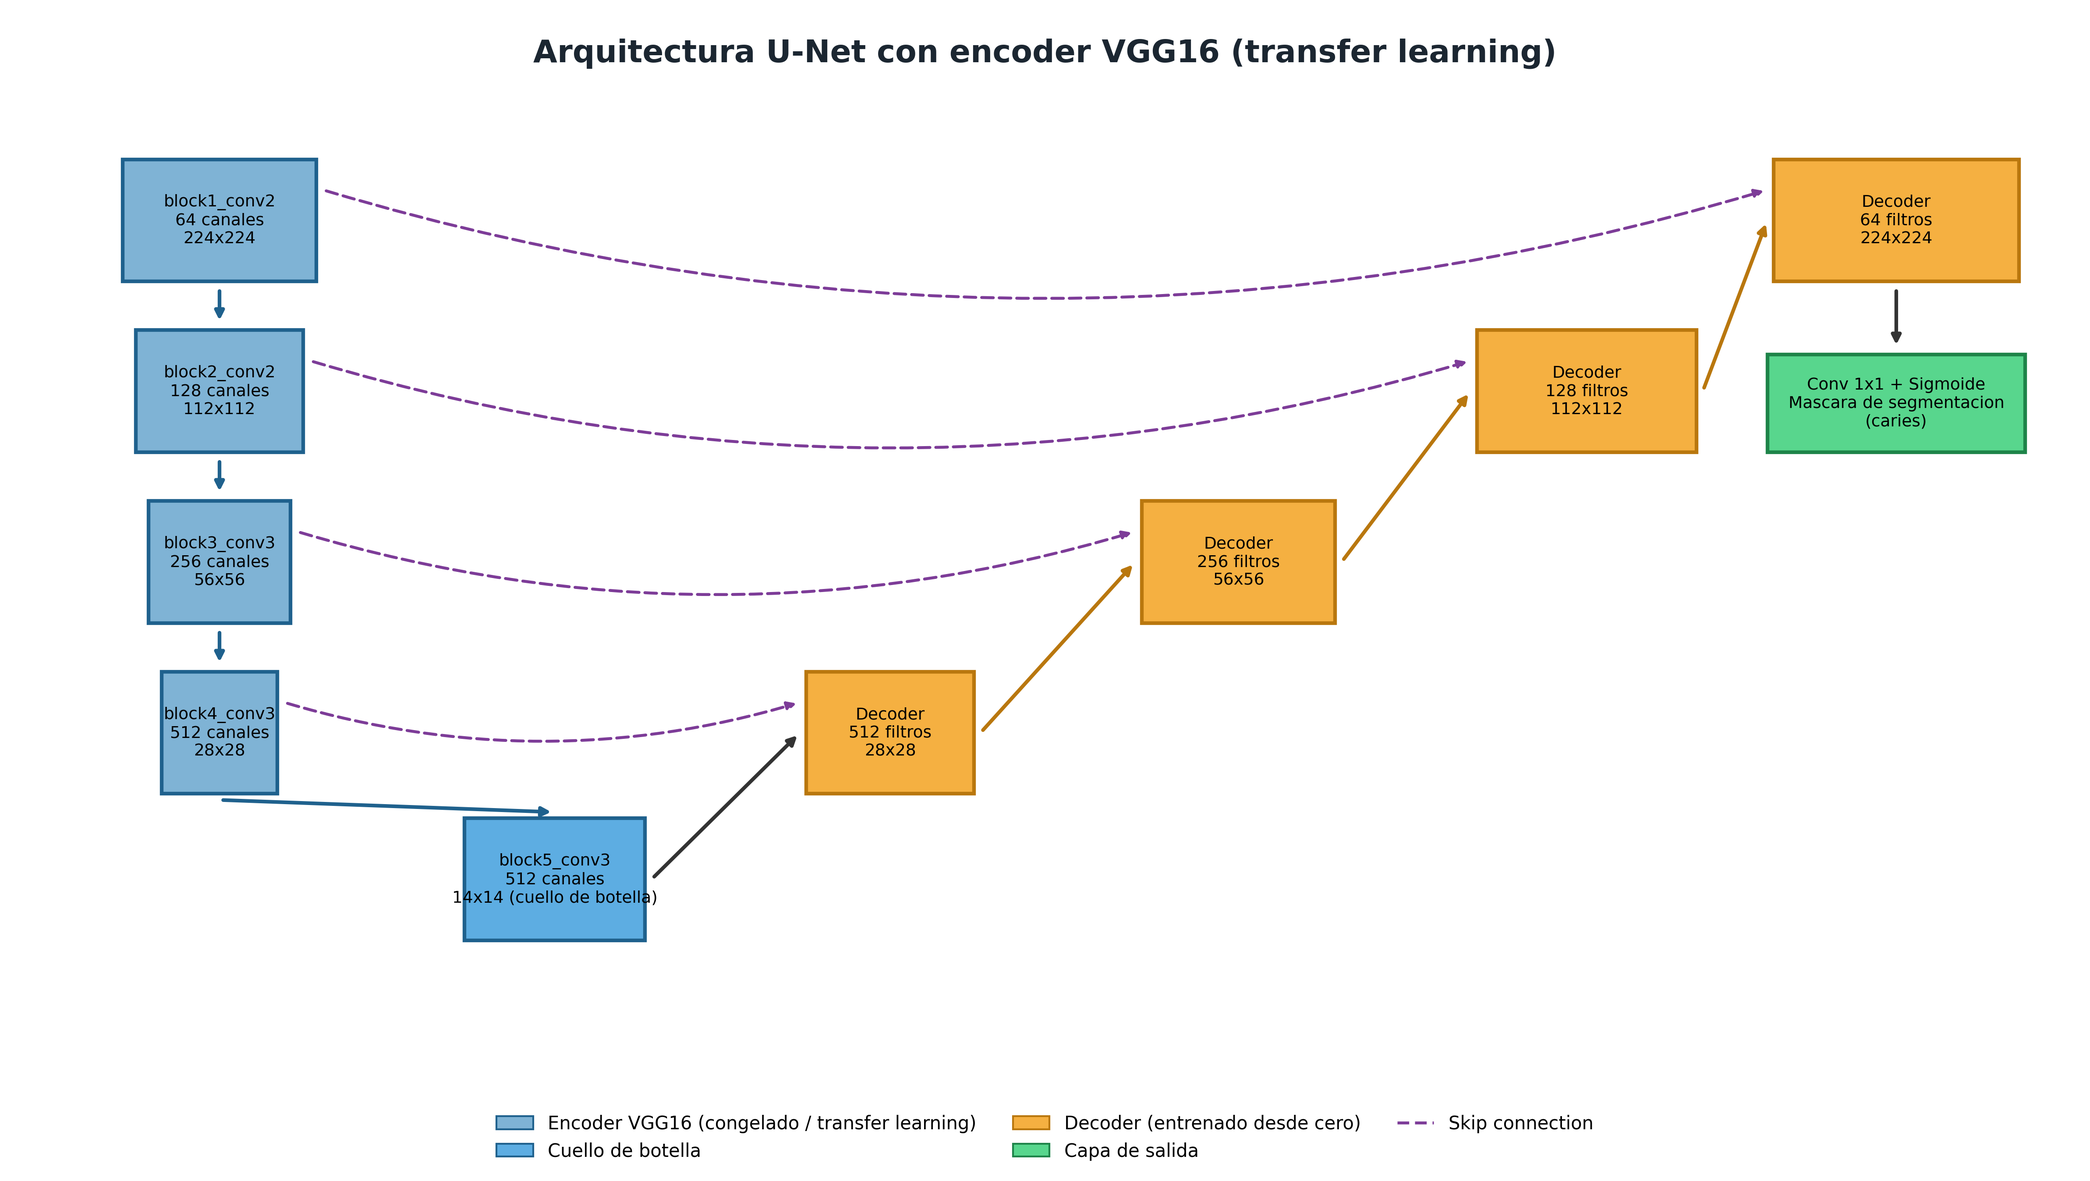
\includegraphics[height=10cm]{diagrama_unet_vgg16.png}
\end{center}

\vspace{0.3cm}
\textbf{Función de pérdida:}
\[
\mathcal{L} = \mathcal{L}_{BCE} + \left(1 - \text{Dice}\right)
\]
donde el Dice coefficient compensa el desbalance entre la clase
``caries'' y el fondo de la imagen.

\vspace{0.3cm}
\textbf{Entrenamiento en dos etapas:}
\begin{enumerate}
  \item \textbf{Transfer learning}: se entrena solo el decoder (encoder congelado).
  \item \textbf{Fine-tuning}: se descongela el último bloque de VGG16
  (\texttt{block5}) con tasa de aprendizaje reducida ($10^{-5}$).
\end{enumerate}
\end{block}

\begin{block}{Resultados}

\begin{center}
% ---- curvas de entrenamiento ----

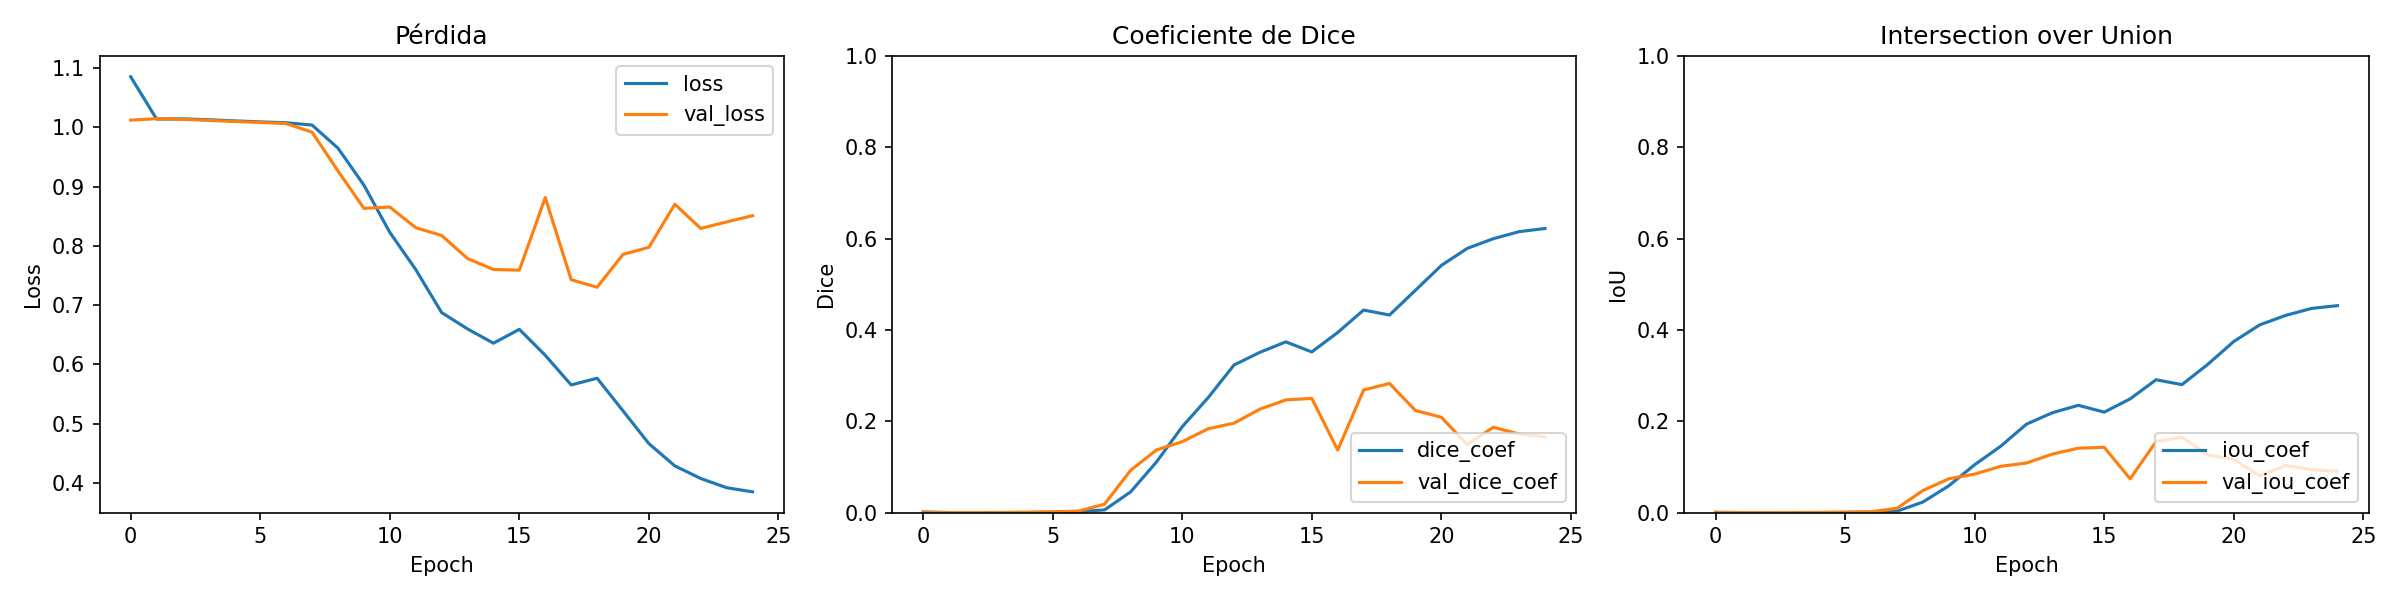
\includegraphics[height=10cm]{modelos.png}
\end{center}

\vspace{0.4cm}
\begin{center}
\begin{tabular}{lcc}
\toprule
\textbf{Métrica} & \textbf{Antes fine-tuning} & \textbf{Después fine-tuning} \\
\midrule
Dice coefficient & 0.2829 & 0.1623 \\
IoU               & 0.1650 & 0.0885 \\
Accuracy          & 0.9979 & 0.9988 \\
\bottomrule
\end{tabular}
\end{center}

\vspace{0.4cm}
\begin{center}
% ----  comparacion visual ----
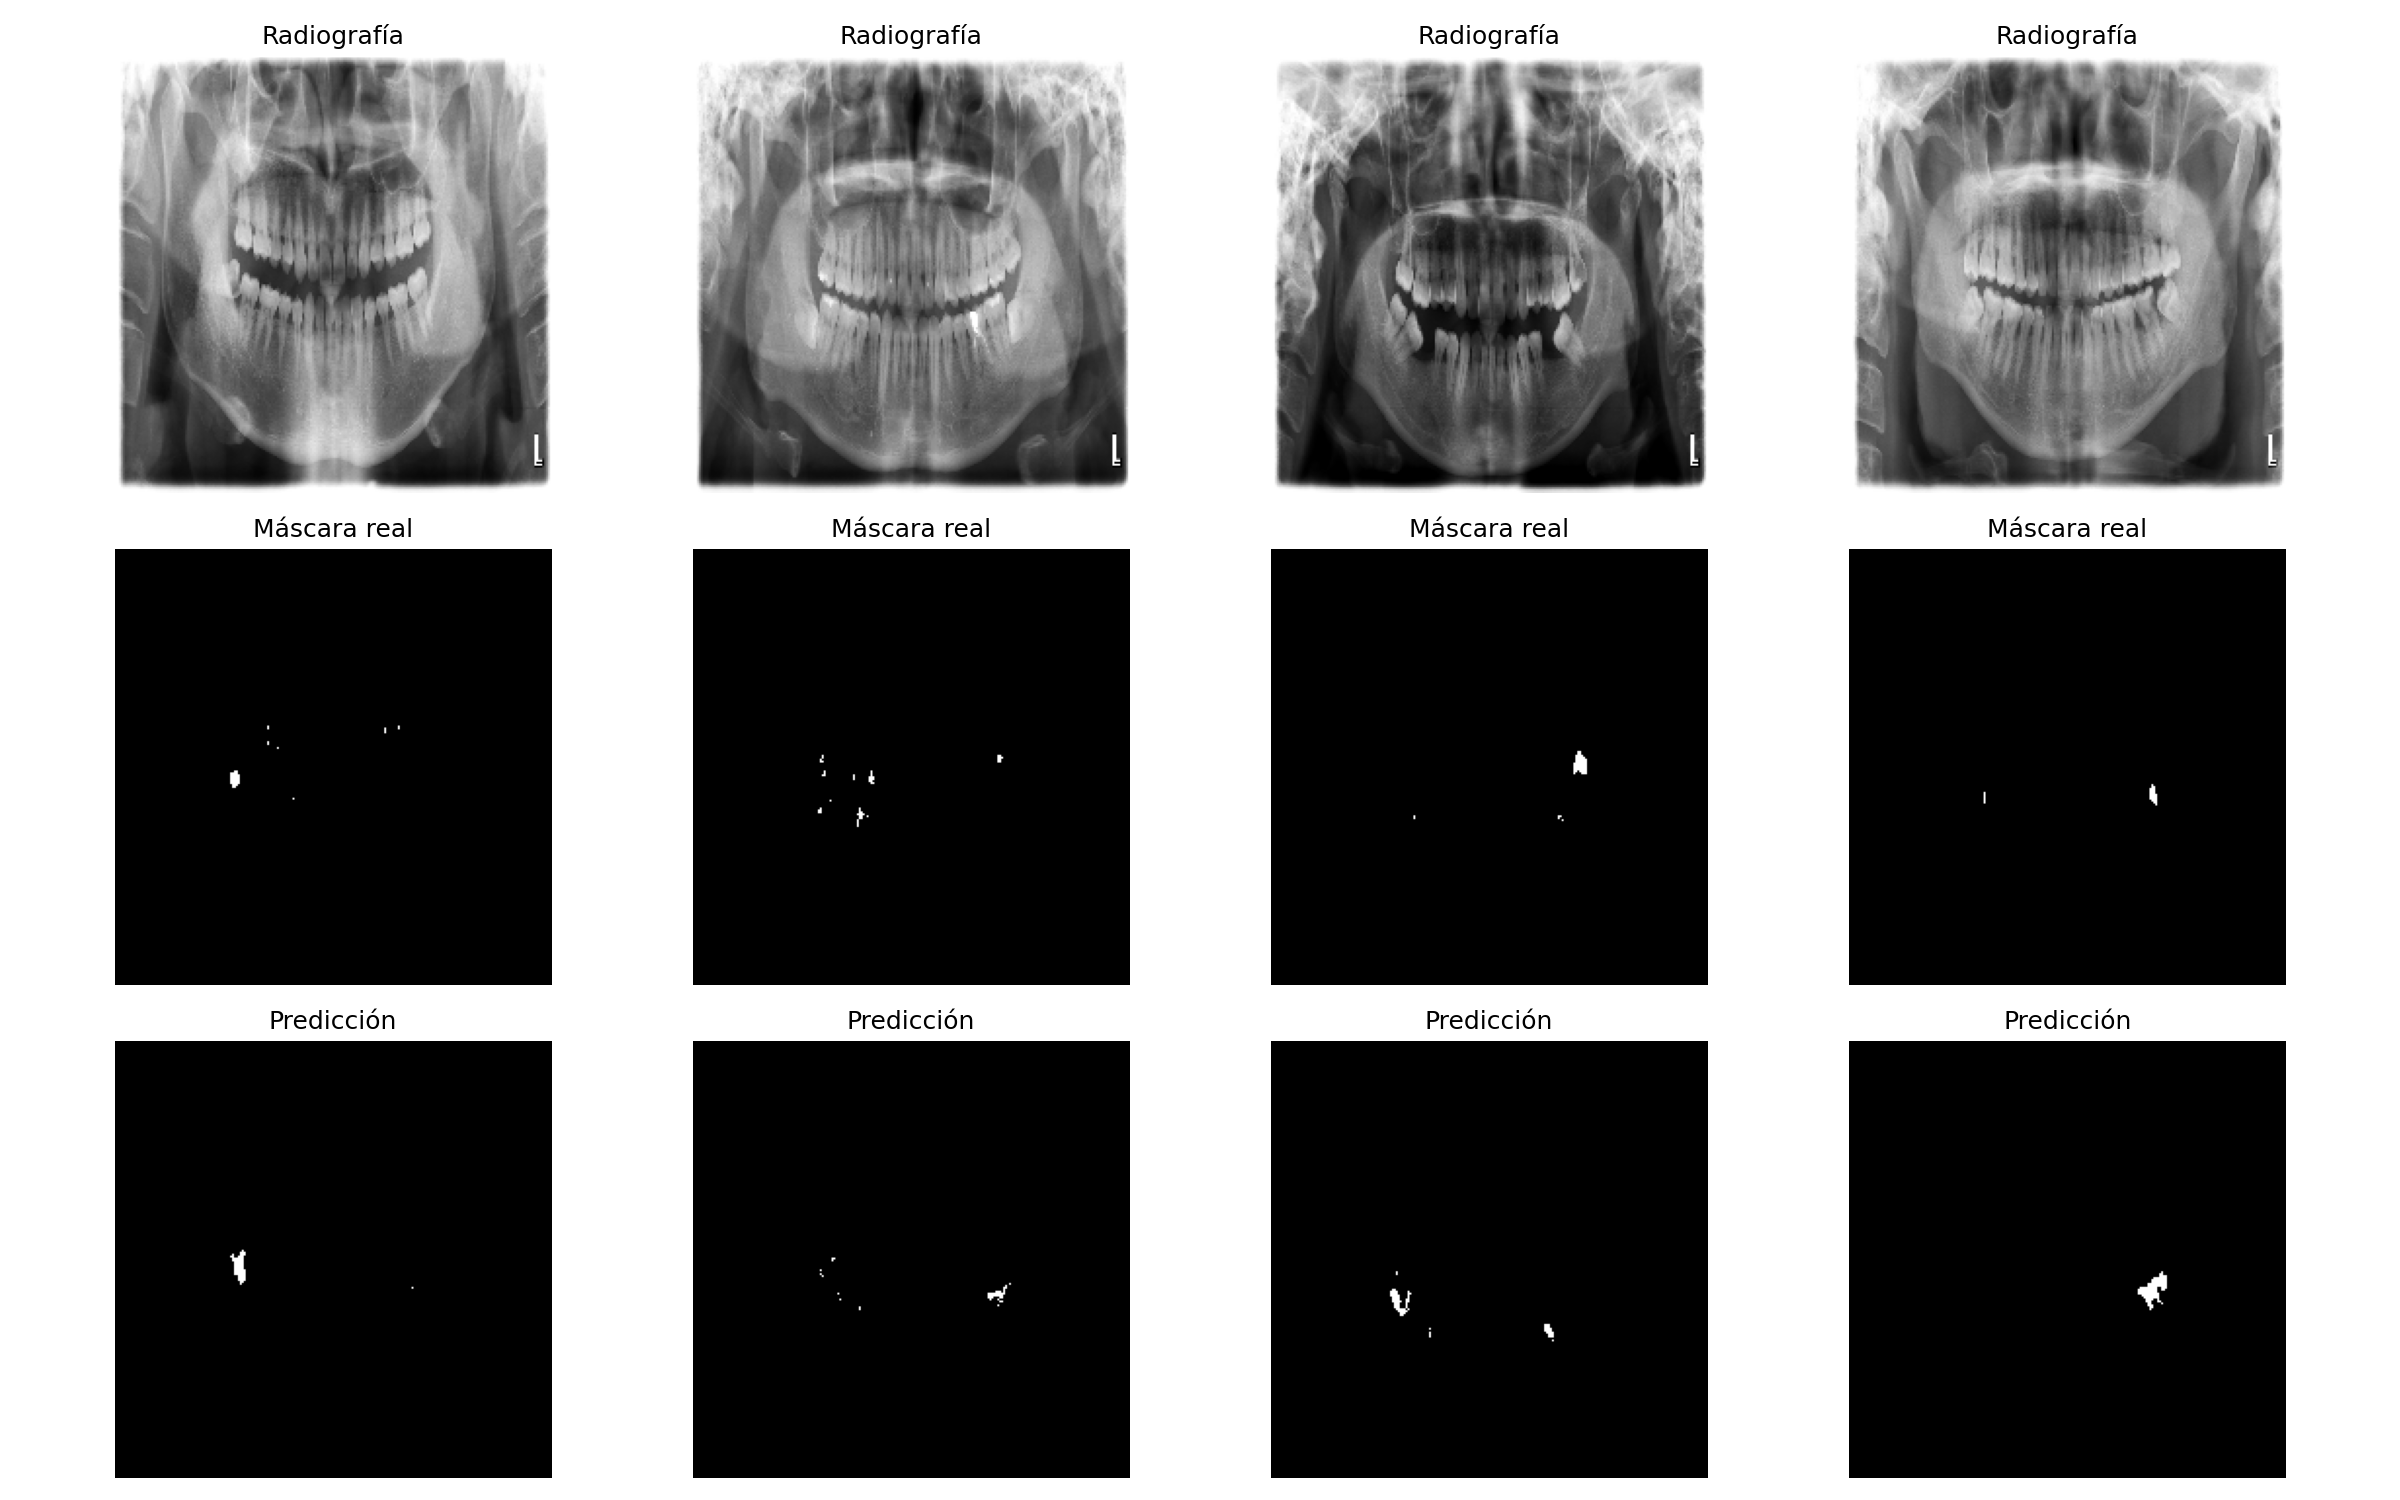
\includegraphics[height=10cm]{predicciones.png}
\end{center}
\end{block}

\begin{block}{Conclusiones}
\textit{[COMPLETAR: resumen de hallazgos principales, por ejemplo el
impacto del fine-tuning sobre el Dice/IoU, la calidad de los bordes
segmentados, y limitaciones asociadas al tamaño del conjunto de datos.]}
\end{block}

\begin{block}{Referencias}
{\footnotesize
Wang, X. et al. (2023). Multi-level uncertainty aware learning for
semi-supervised dental panoramic caries segmentation. \textit{Neurocomputing}, 540.
\\[0.2em]
Ronneberger, O., Fischer, P., \& Brox, T. (2015). U-Net: Convolutional
Networks for Biomedical Image Segmentation. \textit{MICCAI}.
\\[0.2em]
Simonyan, K., \& Zisserman, A. (2014). Very Deep Convolutional Networks
for Large-Scale Image Recognition. \textit{arXiv:1409.1556}.
\\[0.2em]
Repositorio del dataset: \url{https://github.com/Zzz512/MLUA}
}
\end{block}

\end{column}
\end{columns}

\end{frame}
\end{document}
